% Related work: Bitcoin, Namecoin, etc.
\section{State of field}
Standards and technologies for web applications are being rapidly developed, and the boundaries for what is possible to achieve in a web application is being continously pushed by browser vendors and standards groups. Of relevance to Rymd, the Web Real-Time Communications (WebRTC) protocol has become usable for arbitrary data streams in major browsers in 2014. Also of relevance, the still unfinalized Web Crypto API is currently available in an experimental stage in recent months at the time of this writing. The goals of Rymd has thus become technically viable in a web environment as of very recently.

Furthermore, there is currently a lot of work underway in the field of distributed secret communication. Notable projects that share similar ideas or have inspired Rymd are mentioned under Similar technologies. Also worth noting is the new field of cryptocurrencies, which work by distributing a cryptographically based ledger over an entire network. The first and most well-known is Bitcoin, but there are also subsequent currencies that extend the original idea beyond that of a traditional currency to a system that can be used for a wide range of applications. The first worth noting is Namecoin, which adds a global and secure key-value store. Another interesting initiative is Ethereum, a cryptocurrency with contracts that not only allow storage of arbitrary data in the blockchain, but can also be scripted with a Turing complete programming language and can therefore be used to implement arbitrary systems. A system like Ethereum could be very interesting to explore for a project like Rymd, but it is still in such an early stage that it is deemed to unstable to be useful at this point. Namecoin is currently considered a good candidate for key distribution.

\section{Similar technologies}
There is a plethora of disparate technologies for distributing and syncing data between peers that at first glance may look very similar to Rymd. Below are some more well-known and similar pieces of software. The features described will hopefully highlight how they relate to each other and Rymd.
\subsection{Bittorrent Sync}
Bittorrent Sync\cite{BitTorent:2014:Online} is a distributed peer-to-peer multi-way file syncing software using the Bittorrent protocol for file transfers. Synced folders are mapped directly to the underlying file system, and each folder is encrypted using a shared secret key. Public-key cryptography is not employed, and there are only closed-source binary clients using Bittorrent, Incs network available. While they do have a developer API, it requires developer keys issued from Bittorrent Inc.
\subsection{RetroShare}
RetroShare\cite{Retroshare:2014:Online} markets itself as a Friend-2-Friend decentralized communication platform. It uses GPG to create a Web of Trust between peers. It is, however, a very large project: The application provides file-sharing, instant messaging, discussion forums, e-mail, VoIP and group chat. It is open source and distributed as cross-platform binaries.
\subsection{ShareFest}
ShareFest\cite{Sharefest:2014:Online} is a peer-to-peer one-to-many file-sharing web based software using WebRTC data channels. ShareFest can be seen as a more limited and primitive version if what Rymd aims to be: ShareFest can share files over WebRTC channels, but does not accommodate for authentication, persistence or local encryption. It does, however, operate on a mesh network similar to Bittorrent.
\subsection{Freenet}
As one of the first “darknets”, Freenet\cite{Freenet:2014:Online} consists of a distributed, decentralized data store that uploads files with strong anonymity across a network. Each node in the network also acts as a cache for the content stored in the network. Files are generally split up in parts that are distributed, and when fetching files it is unfeasible to determine the origin and sender of the files. Focusing on anonymity, free speech and plausible deniability, the encryption is done in the communication and storage layers. Because of this design, Freenet is quite slow. Files can be retrieved using the cryptographic key used to upload it. Freenet is free software built with Java.
\subsection{Tahoe-LAFS}
Tahoe-LAFS\cite{Tahoe:2014:Online}, or Tahoe Least-Authority Filesystem is a distributed, encrypted and redundant file system. It distributes encrypted files across a predetermined set of servers and allows sharing of both mutable and immutable files. There is a web-interface, but like all other user-interfaces it has to go through a “gateway” where encryption and server-communication is performed. Users will typically run their own gateways and will thus need to accommodate for hosting for them. 
\subsection{Bitmessage}
Bitmessage\cite{Bitmessage:2014:Online} is a P2P distributed messaging system intended to replace e-mail. Public keys of all participants are distributed over the entire network, and can be retrieved using their fingerprints (which are used as addresses). In order to send a message, it is encrypted using the receiver's public key and sent to the entire network. Participants try to decrypt every message, and will so be able to retrieve the ones they can decrypt. Messages are stored in the network for two days. There is thus no way to tie messages to senders and recipients.

\section{WebRTC}
WebRTC is a project which enables real-time communication between browsers\cite{WebRTC:Online}. Through the project, developers are able to create different types of applications which leverage peer-to-peer technology.

To obtain and transfer streaming data WebRTC's functionality is abstracted into three different APIs: \emph{MediaStream}, \emph{RTCPeerConnection} and \emph{RTCDataChannel}\cite{WebRTCBasics:2012:Online}. MediaStream, or \emph{getUserMedia}, consists of synchronized media streams, e.g. synchronized video and sound from a computer's camera and microphone. RTCPeerConnection manages reliable and efficient communication of the data streams. There are a lot going on under the hood that ensures reliability for real time communication even in unstable networks. Furthermore, when a peer connection is present arbitrary data can be sent by leveraging RTCPeerConnection with RTCDataChannel.

\subsection{RTCDataChannel}
The RTCDataChannel demonstrated the capabilities that Rymd desired. Data transfers are secured with the DTLS (Datagram Transport Layer Security) protocol. The DTLS protocol is based on the TLS (Transport Layer Security) protocol, the main difference being that DTLS is constructed for datagrams while TLS is used for more reliable transport protocols such as TCP.

Before a connection can be initiated between peers, one of two parts must extend an offer which contains data describing the connection to the other part - this is often referred to as the signaling phase. The signaling phase requires a channel where the offer can be negotiated - it is usual for the channel to be a dedicated signaling server, but examples of a more serverless approach can be found\cite{webrtcsignalserver}. The standard does not provide any recommendations regarding the choice of signaling channel and protocol - this is for developers to decide. The connection phase is then handled by ICE (Interactive Connectivity Establishment).

\subsection{ICE}
ICE is a framework with the objective of connecting peers\cite{WebRTCBasics:2012:Online}. Since computers today are usually behind NAT gateways they are using different IP-addresses in their private network and the same IP-adress publicly to the access the Internet. This poses difficulties when trying to achieve a peer-to-peer connection.

\begin{figure}[h]
\centering
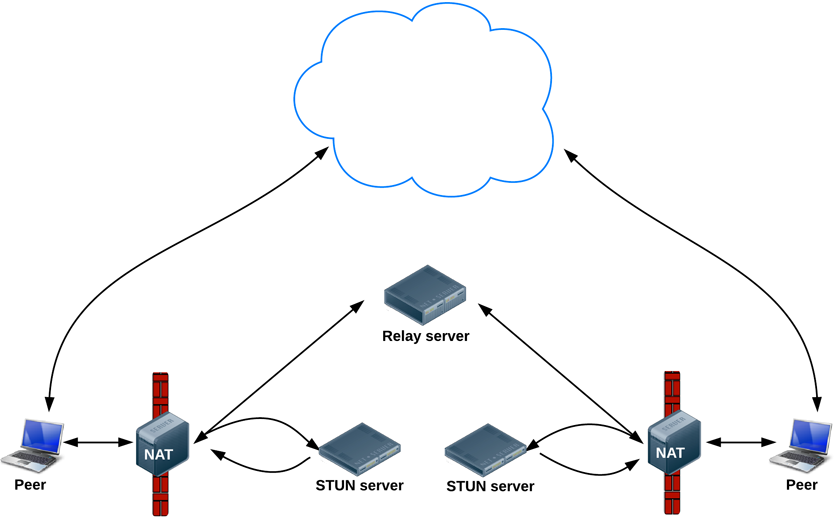
\includegraphics[width=\textwidth,height=0.25\paperheight,keepaspectratio
]{figures/ICE}
\caption{The different ways for ICE to find network interfaces and ports \cite{WebRTCBasics:2012:Online}}
\label{fig:ICE}
\end{figure}

ICE decides between different ways of achieving a connection and chooses the one with the lowest latency\cite{WebRTCBasics:2012:Online}. At first ICE tries to connect peers cleanly through UDP and STUN (Session Traversal Utilities for NAT). STUN servers are simple, cheap to run and enables a peer behind a NAT to discover its public adress and port. When the IP-addresses are known data doesn't need to go througn the server but instead flows directly between the peers. However, if it is not possible to establish a connection ICE attempts to use TCP instead of UDP: first HTTP and then HTTPS. If STUN doesn't work, probably because of firewalls and more advanced NAT systems, ICE uses cloud fallback in the form of a TURN (Traversal Using Relay NAT) server. This connection isn't peer-to-peer since the data needs to go through the server and because of this it is also slower than the previous alternatives. But it allows a connection to be made under almost any condition. 

\section{IndexedDB}
% More stuff here: http://www.cms.livjm.ac.uk/pgnet2012/Proceedings/Papers/1569607913.pdf
The IndexedDB is a transactional, indexed client side database capable of storing different types of data structures with an asynchronous API. IndexedDB is actively developed and implemented in the latest versions of Mozilla Firefox, Google Chrome, Microsoft Internet Explorer and Opera: its specification is a Candidate Recommendation by the W3C, as of July 2013\cite{IndexedDB:Online}:

\begin{quote}
This document defines APIs for a database of records holding simple values and hierarchical objects. Each record consists of a key and some value. Moreover, the database maintains indexes over records it stores. An application developer directly uses an API to locate records either by their key or by using an index. A query language can be layered on this API. An indexed database can be implemented using a persistent B-tree data structure.
\end{quote}

\subsection{Basic structure}
% Cursors, Object Stores, Indexes
Due to IndexedDB's object-oriented nature, a database includes a set of \emph{object stores}, which act like tables in relational database management systems. An object store can hold \emph{objects} of different types, including binary data and Javascript primitives and objects. Each object has a \emph{key} (either specified by the developer from the object's properties, or automatically generated and managed by the database) that is used for indexing and retrieving records. One or several \emph{indexes} can be created on a store from an object's properties for quick querying. A \emph{cursor} is used to iterate on the resulting set of objects from a query on the store.

% Async API
% -----------
% Requests, Callbacks, Events, NoSQL
The asynchronous API might include complex patterns if the developer is not used to NoSQL structures. Unlike WebSQL, IndexedDB does not support SQL, and instead exposes ways for querying and manipulating data via \emph{requests} and \emph{transactions} (see section~\ref{subsec:security}). A positive facet of the rejection of SQL in favor of NoSQL is the prevention of SQL injection attacks, but with the cost of a steeper learning curve for already experienced database developers. Queries to the database will not yield the resulting data set: instead requests are returned, which will trigger \emph{events} for when the operation is finished. When an event is triggered a \emph{callback} can be passed to handle the scenario and use the data. This goes well with the asynchronous nature of Javascript, where events and callbacks are used heavily. Using asynchronous passing of callbacks prevents the program execution to block at a line when a potentially heavy operation is called. The Javascript code snippets below show the difference in synchronous and asynchronous calls.

\begin{Code}
\begin{lstlisting}[caption=Synchronous call]
// Fetch a record with id 10 from a database and store in variable
var result = DB.find(10);
\end{lstlisting}

\begin{lstlisting}[caption=Asynchronous call]
/*
  Request a record with id 10 from a database, continue execute other code,
  and handle result of the database operation in callback when it has finished
*/
var request = DB.find(10);

request.onsuccess = function(evt) {
  var result = evt.result;
};
\end{lstlisting}
\end{Code}

\subsection{Security and reliability}
\label{subsec:security}
IndexedDB is built on a transactional model, which implicates that all commands runs inside a transaction context. Transactions have a certain lifetime, and cannot be used after its expiration. This transactional model is especially useful for when several instances of a client application is using the same database and issuing commands: without transactions, concurrency problems and other collisions might occur with data loss as a result. Transactions are able to abort and be rolled back to the state of the database before the transaction was started.

Kimak, Ellman and Laing highlight four important aspects of securing a IndexedDB driven application in their \emph{An Investigation into Possible Attacks on HTML5 IndexedDB and their Prevention}\cite{IndexedDBSecurity:2012:Online}:

\begin{itemize}
  \item Client side data encryption
  \item Input validation
  \item SOP (Same-Origin Policy)
  \item Code analysis
\end{itemize}

The database in IndexedDB does not include any kind of bundled encryption or validation, which means it is the developer's responsibility to sanitize and encrypt sensitive data before inserting into the store. Encryption is vital for the scenario where the contents of the database is compromised: the attacker must have access to the encryption key in order to read the information in plain text. Validation is needed if malicious content, such as Javascript, is inserted as the data fields in the store and then will be executed at a later stage.

The \emph{Same Origin Policy} is used in IndexedDB. An origin is the transfer protocol, the domain, and the port number. Thus every database is associated with an origin, which implicates certain security aspects: an application in \emph{http://domain.com/subdir} may retrieve data from \emph{http://domain.com/subdir/dir} since they have the same origin, but cannot retrieve data from \emph{https://domain.com:3000} due to the different protocol and port number. This is a layer of protection against Cross Site Scripting (XSS) attacks, even though there is no prevention against XSS holes in the other parts of the application (the database might be compromised due to malicious scripts injected elsewhere).

Code analysis is divided into \emph{static} and \emph{dynamic} analysis. Static analysis is the analysis of the to-be insterted data in order to detect malicious material. Dynamic analysis is the analysis of executed programs, and can according to \cite{IndexedDBSecurity:2012:Online} be done by checking the call from the web application to the database and on success, the database operation can be performed.

\section{Namecoin}
A phenomenon that has been on the rise during recent years is that of cryptocurrencies such as Bitcoin \cite{CryptoCoinInsider:2014:Online}. Each participant in the Bitcoin network keeps a ledger of all transactions throughout the history of the network. In order for a transaction to be deemed valid, it needs to be included in a cryptographically signed block together with a salt by one of the nodes, with a hash that has a special format. It is this brute-force search for salts that generate these hashes that are called \emph{mining} and constitute the work done by \emph{miners} to keep the network running. As an incentive, each verified block also includes a reward to the miner that first finds it and submits it to the blockchain\cite{InternetForBeginners:2014:Online}. In effect, all transactions ever made are publicly available and tracked so that anyone can confirm their validity. This prevents forgery and double-spending of bitcoins.

Another cryptocurrency is Namecoin\cite{CryptoCoinInsider:2014:Online}. Namecoin is essentially a fork of Bitcoin with new transaction types that allows its blockchain to be utilized as a distributed key-value store. Although similar in nature to Bitcoin, its main purpose is to be used as a decentralized domain name system (DNS), rather than as a monetary currency.

With a decentralized DNS such as Namecoin, top level domains (such as \emph{.com} or \emph{.se}) can exist without being controlled by any central authority \cite{CryptoCoinInsider:2014:Online}. Also, the DNS lookup tables where domain names and their IP addresses are stored are shared in a peer-to-peer manner. The only necessary condition for these domains to be accessible is that there are participants willing to run the DNS server software. Although mainly intended to be used as a DNS, it contains several namespaces where arbitrary strings such as public cryptographic keys can be stored.
